\section{Product Concept}

This section describes the purpose, use, and intended user audience for the laser harp. The laser harp is a musical instrument designed to provide an innovative and engaging way to create music using laser technology. Users of the laser harp will be able to produce sounds by interrupting laser beams, simulating the plucking of strings on a traditional harp. This section provides a high-level statement of the product concept, outlining what it is intended to do and how it is intended to be used.

\subsection{Purpose and Use}
The laser harp is designed to provide an interactive musical experience by using laser beams as virtual strings. When a laser beam is interrupted, the system detects the interruption and plays a corresponding musical note. The purpose of the laser harp is to offer a unique and modern approach to playing music, combining elements of traditional string instruments with advanced technology. It is expected to be used in educational settings to inspire interest in STEM subjects, as well as by musicians and hobbyists looking for an innovative way to create music.

\subsection{Intended Audience}
The intended audience for the laser harp includes educational institutions, music enthusiasts, and hobbyists. In educational settings, the laser harp can be used as a tool to engage students in learning about music, electronics, and programming. Music enthusiasts and hobbyists will appreciate the creative possibilities offered by the laser harp, as it provides a new way to experiment with musical composition and performance. The product is designed for general use and can be integrated into various educational and recreational activities.

\begin{figure}[h!]
	\centering
   	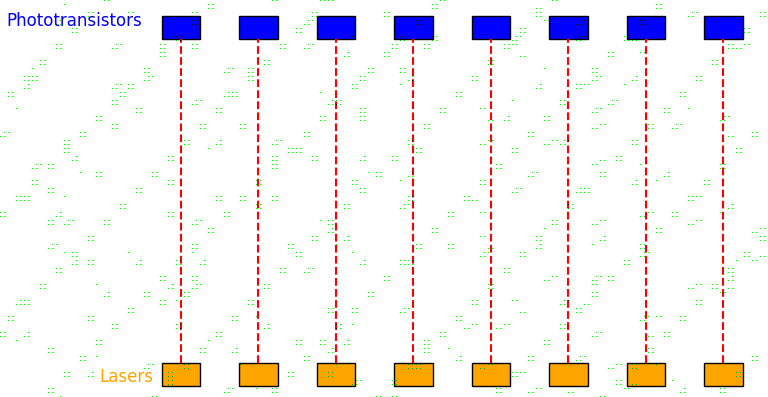
\includegraphics[width=0.60\textwidth]{images/Design}
    \caption{Laser Harp conceptual drawing}
\end{figure}
